\label{chapter:resultados}
O presente capítulo consiste em apresentar a execução e resultado referente ao método proposto, visando avaliar de forma experimental o INEXT para identificação e localização de objeto em edifícios utilizando RFID.

\section{Planejamento e projeto dos experimentos}
Esta avaliação experimental consiste em avaliar o INEXT, tendo como questões principais a identificação e localização de objetos em ambientes confinados e então o gerenciamento dos objetos. Em virtude disso, foi definida as seguintes questões:
\begin{itemize}
    \item[QP1]: O sistema proposto consegue identificar e localizar objetos no âmbito confinado?
    \item[QP2]: O método proposto agiliza o gerenciamento dos objetos em edifícios?
    
\end{itemize}{}
\par 
Objetivando responder tais questões, foram utilizados um Arduíno Nano e um computador comunicando-se através da porta serial para simular a segunda sala, pois não disponhamos de duas placas NodeMcu, em seguida usamos um \textit{script} na linguagem Python para ler os dados da porta serial, criar um objeto JSON e enviar para o servidor, tais código estão disponíveis no repositório dentro da pasta ''prototype\_arduino''. O computador utilizado possui $4GB$ de memória RAM, processador Intel Core $i5-2500$, HD de $500GB$ e sistema operacional \textit{Windows} $7$ \textit{Professional} $64Bits$.  Os protótipos podem ser visualizados nas \autoref{fig:prototipo_arduino} e \autoref{fig:prototipo_nodemcu}. 

\begin{itemize}
    \item 3.3V - conectado ao pino de 3.3v no Arduino, essa conexão faz a alimentação do leitor RFID;
    \item RST (\textit{Reset})- conectado ao pino 9 do Arduino;
    \item GND (\textit{graduated neutral density filter}) - conectado ao pino GND do Arduino;
    \item NC/IRQ (\textit{Interrupt Request})- não utilizado;
    \item MISO (\textit{Master In Slave Out}) - conectado ao pino 12;
    \item MOSI  (\textit{Master Out Slave In}) - conectado ao pino 11;
    \item SCK  (\textit{Serial Clock}) - conectado ao pino 13;
    \item SDA/ SS (\textit{Serial Data Line/ Select Slave}) - conectado ao pino 10.
\end{itemize}    

\begin{figure}[H]
              \caption{\label{fig:esq_conexoes_arduino}{Esquema de Conexões Arduíno Nano}}
              \centering
              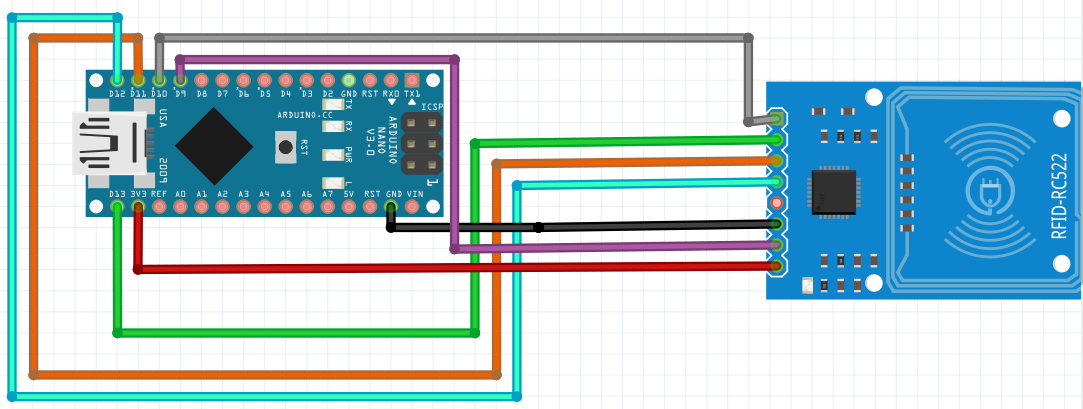
\includegraphics[width=1\textwidth]{Figuras/esquema_de_conexoes1.PNG}
              \legend{Fonte: Própria}
\end{figure}
\begin{figure}[H]
              \caption{\label{fig:prototipo_arduino}{Protótipo Arduíno Nano}}
              \centering
              \includegraphics[width=1\textwidth]{Figuras/prototype_arduino.png}            \legend{Fonte: Própria}
\end{figure}\begin{figure}[H]
              \caption{\label{fig:prototipo_nodemcu}{Prototipo NodeMcu}}
              \centering
              \includegraphics[width=1\textwidth]{Figuras/prototype_nodemcu.png}
              \legend{Fonte: Própria}
\end{figure}
\par
Para a simulação do servidor, foi utilizado um notebook com $6GB$ de memória RAM, processador Intel Core $i5-4200$, HD de $750GB$, placa de video GeForce $720M$ de $2GB$ de memória dedicada e sistema operacional \textit{Windows 10 Home Single Language}. A rede LAN utilizada foi criada através de um roteador \textit{TP-LINK} modelo $TL-WR720N$. Também foram utilizadas quatro etiquetas RFID passivas, cada uma dessas etiquetas representa um objeto diferente para a simulação.

\section{Execução dos experimentos e Análise dos Resultados}
A execução do experimento aconteceu no cenário apresentado na \autoref{fig:cenario}, como havia sido mencionado anteriormente, foi simulado duas salas e quatro objetos rastreáveis em um edifício. Foram executados os seguintes testes: (1) localização e identificação dos objetos, (2) restrição de objeto e notificação ao violar restrição e (3) gerenciamento dos objetos.
\begin{figure}[H]
              \caption{\label{fig:cenario}{Cenário de simulação}}
              \centering
              \includegraphics[width=1\textwidth]{Figuras/cenario.png}
              \legend{Fonte: Própria}
\end{figure}
\par
Após a execução dos testes, foi constatado que o INEXT consegue localizar objetos em ambientes confinados, porém o sistema não proporciona a posição real do objeto no ambiente, o sistema também foi capaz de identificar os objetos mas essa etapa ainda ocorre de maneira manual necessitando ser realizada por usuários.

\par
Os testes seguintes foram a criação de restrição para objetos e verificar se os todos usuário eram notificados quando a restrição fosse violada, o sistema foi capaz de notificar os usuários através do e-mail e na tela inicial do sistema. O ultimo teste foi a realização do levantamento de todas as salas e objetos que cada sala possui, o INEXT foi capaz de realizar essa tarefa e gerou logs para todas as operações realizadas.
